%% ICRAT 2024.tex
%% V1.0
%% 2024/01 
%% created by Thinh Pham, modified from ATM2023.tex by Ramon Dalmau

\documentclass[conference, letter]{IEEEtran}
\IEEEoverridecommandlockouts

% *** GRAPHICS RELATED PACKAGES ***
%
\ifCLASSINFOpdf
  \usepackage[pdftex]{graphicx}
  % declare the path(s) where your graphic files are
  %\graphicspath{}
  % and their extensions so you won't have to specify these with
  % every instance of \includegraphics
  \DeclareGraphicsExtensions{.pdf,.jpeg,.png}
\else
  % or other class option (dvipsone, dvipdf, if not using dvips). graphicx
  % will default to the driver specified in the system graphics.cfg if no
  % driver is specified.
  % \usepackage[dvips]{graphicx}
  % declare the path(s) where your graphic files are
  % \graphicspath{{../eps/}}
  % and their extensions so you won't have to specify these with
  % every instance of \includegraphics
  % \DeclareGraphicsExtensions{.eps}
\fi

% *** PACKAGES ***
\usepackage{cite}
\usepackage{amsmath,amssymb,amsfonts}
\usepackage{algorithmic}
\usepackage{graphicx}
\usepackage{textcomp}
\usepackage[left=1.29cm, right=1.29cm, top=1.9cm, bottom=4.29cm]{geometry}
% \usepackage{caption}
\usepackage{enumitem}
\usepackage{anyfontsize}
\usepackage{lipsum}
\usepackage{hyperref}

% \captionsetup[table]{format=plain,labelformat=simple,labelsep=period, textfont=sc}%
\setlength{\columnsep}{7mm}

% *** HEADER ***
\usepackage{fancyhdr}
\pagestyle{fancy}
\lhead{Student Research Task 2025/26}
\rhead{Chair of Air Transport and Logistics}
\renewcommand{\headrulewidth}{0pt}

% *** CHANGE FIGURE LABEL ***
\makeatletter
\renewcommand{\fnum@figure}{Figure \thefigure}
\makeatother

% *** TITLE ***
\title{ {Energy Consumption Modeling for UAVs Based on Flight Data and Mission Parameters}
\vspace{0.5cm}
}

% *** AUTHORS ***
\author{\IEEEauthorblockN{Research Task Group 4, \textit{Masters in Air Transport and Logistics}}
\IEEEauthorblockA{Chair of Air Transport and Logistics \\
TU Dresden, Dresden, Germany \\}
}

\renewcommand\IEEEkeywordsname{Keywords}
\IEEEaftertitletext{\vspace{-1\baselineskip}}

% *** DOCUMENT ***
\begin{document}

\maketitle
\thispagestyle{fancy}

\noindent \begin{abstract}
This study presents a comprehensive analysis of UAV energy consumption using a high-fidelity, publicly available dataset from $209$ autonomous flights of a DJI Matrice 100 quadcopter, collected over seven months under diverse operational and environmental conditions. The dataset enables robust empirical investigation of power dynamics across varying payloads, altitudes, and flight phases. Histogram analysis of vertical velocity, horizontal speed, and power consumption reveals distinct multimodal distributions, which inform the selection of phase-specific thresholds:
$\pm0.6~\text{m/s}$ for vertical motion, $0.3~\text{m/s}$ for horizontal speed, and $50~\text{W}$ for power. These thresholds support a robust, threshold-based classification of flight phases—Taxi, Hover, Cruise, Climb, Descent, and Other—ensuring physically meaningful segmentation of UAV flight data.
A physics-based, segment-wise power model is developed using actuator disk theory and phase-dependent efficiency estimates. The model demonstrates strong performance across climb, descent, and cruise phases, with MAPE below $12\%$ in cruise flight, validating its ability to capture key aerodynamic and propulsion dynamics under steady-state conditions.
Complementing this, a Random Forest regression model is trained on $19$ flight-state features—including velocity, wind conditions, attitude, and flight mode indicators—achieving an
$R^2$ score of $0.941$ and sub-$50~\text{W}$ MAE across all phases. The model exhibits superior predictive accuracy, reducing error by up to $50\%$ compared to the physics-based approach, and accurately captures transient power dynamics during complex maneuvers.
However, a critical trade-off emerges: while the data-driven model excels in accuracy and temporal fidelity within its training domain, it exhibits unphysical extrapolation and limited interpretability. In contrast, the physics-based model, though less accurate in complex regimes, offers greater transparency and robustness to out-of-distribution conditions.

\end{abstract}

\vspace{0.3cm}

\begin{IEEEkeywords}
UAV energy consumption, Physics-based model, Data-driven modeling, Model comparison, Flight data analysis, Machine learning for UAVs
\end{IEEEkeywords}
% \section*{Abbreviations and Symbols}
% \begin{table}[htbp]
\centering
\caption{List of Abbreviations}
\begin{tabular}{lll}
\textbf{Abbreviation} & \textbf{Description} & \textbf{Units} \\
$ \text{RoC} $ & Rate of climb & m/s \\
$ \text{RoD} $ & Rate of descent & m/s \\
\end{tabular}
\label{tab:abbreviations}
\end{table}

\begin{table}[htbp]
\centering
\caption{List of Symbols Used}
\begin{tabular}{lll}
\textbf{Symbol} & \textbf{Description} & \textbf{Units} \\
$ P_{\text{real}} $ & Measured battery power & W \\
$ P_{\text{model, phys}} $ & Predicted battery power (physics model) & W \\
$ P_{\text{mech, base}} $ & Base mechanical power (segment-wise) & W \\
$ P_{\text{hover, base}} $ & Hover-induced power & W \\
$ v_{\text{air}} $ & Airspeed & m/s \\
$ v_z $ & Vertical speed & m/s \\
$ v_x $ & Horizontal speed & m/s \\
$ v_i $ & Induced velocity & m/s \\
$ v_h $ & Hover velocity & m/s \\
$ m_0 $ & Empty mass & kg \\
$ \text{payload} $ & Payload mass & kg \\
$ m $ & Total mass ($m_0$ + payload) & kg \\
$ g $ & Gravitational acceleration & m/s$^2$ \\
$ \rho $ & Air density & kg/m$^3$ \\
$ R_{\text{prop}} $ & Rotor radius & m \\
$ A_{\text{rot}} $ & Single rotor disk area & m$^2$ \\
$ A_{\text{tot}} $ & Total rotor disk area & m$^2$ \\
$ S_{\text{ref}} $ & Reference area & m$^2$ \\
$ C_d $ & Drag coefficient & -- \\
$ \eta_s $ & Segment-wise efficiency & -- \\
$ s $ & Set of flight phase (hover, climb, etc.) & -- \\
$ z_{\text{max}} $ & Maximum altitude during flight & m \\
\end{tabular}
\label{tab:abbreviations}
\end{table}

\section{Introduction}
Energy consumption modeling is fundamental for ensuring the safety, reliability, and efficiency of Unmanned Aerial Vehicle (UAV) operations \cite{ren2025, muli2022, zhang2021, dorling2017}. Because drones have limited battery capacity and short endurance, often limited to 20-30 minutes, accurately predicting power demand is vital for mission planning and range estimation \cite{ren2025, muli2022, conte2022, rodrigues2021}. The sources identify four primary categories of factors that influence a drone's energy usage: drone design (e.g., weight, battery efficiency, rotor size), operating environment (e.g., wind conditions, air density, temperature), drone dynamics (e.g., flight speed, acceleration, angle of attack), and delivery operations (e.g., payload weight) \cite{ren2025, muli2022, zhang2021, patterson2018}.

\subsection{State of the art}
The methodological landscape of energy modeling is generally divided into two paradigms. First, theoretical/physics-based models, these utilize fundamental principles of flight to calculate the energy required to overcome forces such as gravity and aerodynamic drag \cite{zhang2021, rodrigues2021}. These range from simple integrated models based on lift-to-drag ratios to complex component models that separately account for induced power (to maintain lift), parasite power (to overcome air resistance) and profile power (to overcome rotational drag on propeller blades) \cite{bruehl2021,zhang2021}.

Second, data-driven/Machine Learning Models, these leverage architectures such as Long Short-Term Memory (LSTM), Bi-LSTM and Decision Trees to learn complex temporal patterns from empirical flight data \cite{ren2025, muli2022, gora2022, fatima2022}. According to the sources, these "black-box" approaches can often outperform traditional mathematical models by capturing non-linearities and environmental uncertainties without requiring detailed knowledge of a drone's internal construction \cite{muli2022, gora2022}.

A significant challenge highlighted in the sources is the lack of consensus on a universal model \cite{muli2022, zhang2021}. Comparative studies show that different modeling approaches can produce energy consumption estimates that vary by a factor of 3 to 5, even when using identical input parameters and trajectories \cite{ren2025, muli2022, rodrigues2021}. Furthermore, accurate modeling requires analyzing distinct flight regimes, as energy intensive maneuvers like vertical takeoff can account for a substantial portion of total trip energy, sometimes as much as 36\%—compared to horizontal cruise flight \cite{rodrigues2022}. Therefore, high-fidelity modeling must integrate real-world environmental data, such as wind vectors and actual battery voltage drops, to provide the predictive precision necessary for modern UAVs.

\subsection{Structure of the document}
The work begins in section \ref{data_analysis} with a detailed account of data acquisition and analysis, leveraging a publicly available dataset from 209 autonomous flights of a DJI Matrice 100 quadcopter, collected over seven months under diverse operational and environmental conditions \cite{rodrigues2021}. Building on this, the section \ref{flight_phases} defines flight phases through a threshold-based classification scheme, using statistical analysis of vertical velocity, horizontal speed, and power to distinguish between Taxi, Hover, Cruise, Climb, Descent, and Other states, ensuring physically meaningful segmentation of flight data. A physics-based power model is then developed in section \ref{Physic_model} using actuator disk theory and phase-dependent efficiency estimates, providing a transparent, first-principles framework for predicting electrical power consumption during steady-state flight. Complementing this, a Random Forest regression model is introduced in section \ref{data_driven} as a data-driven alternative, trained on 19 flight-state features—including velocity, wind, attitude, and flight mode indicators—to capture complex, non-linear relationships in energy demand. The two models are rigorously validated and compared in section \ref{task_04} using standard error metrics across all flight phases, revealing the superior accuracy of the data-driven approach while also highlighting its limitations in extrapolation and interpretability as described in section \ref{task_05}. 


\section{Data acquisation and analysis}
\label{data_analysis}
\subsection{Data acquisition}
The dataset used in this study is derived from the publicly available \textit{In-flight positional and energy use dataset of a DJI Matrice 100 quadcopter for small package delivery}, published by Rodrigues et al.~\cite{rodrigues2021} in \textit{Scientific Data}. This comprehensive dataset was collected over a period of seven months (April to October 2019) at an open-field test site in Penn Hills, Pennsylvania, USA (40.465690° N, 79.788281° W), under a variety of operational and environmental conditions. The data were gathered from a total of 209 autonomous flights, comprising 195 flights with active cruise phases and 14 additional hover/idle recordings, resulting in a cumulative flight duration of 10 hours and 45 minutes and a total flight distance of approximately 65 kilometers.

The experimental platform was a DJI Matrice 100 (M100) quadcopter \cite{dji2016}, a fully programmable multirotor UAV equipped with a custom sensor suite for high-resolution data acquisition. The airframe, with a total takeoff mass of 3.68 kg (unloaded), was outfitted with a payload system capable of carrying 250 g and 500 g packages, enabling the study of payload-dependent energy consumption. The vehicle was autonomously controlled via a custom Graphical User Interface (GUI) using the DJI SDK, following a predefined triangular flight path with variable cruise altitudes (25 m, 50 m, 75 m, and 100 m), ground speeds (4 m/s, 6 m/s, 8 m/s, 10 m/s, and 12 m/s), and payload masses. Each unique combination of these parameters was repeated at least three times to ensure statistical robustness and data consistency.

The dataset is publicly available under a Creative Commons Attribution 4.0 International License, and the associated codebase is released under the BSD license. This dataset provides a rare, high-fidelity, and well-documented resource for empirical modeling of UAV energy consumption, enabling validation of theoretical models and development of data-driven predictive systems such as the Random Forest model employed in this study.

\subsection{Data preparation and cleaning}
The raw flight data from the DJI~100 were reviewed and cleaned before analysis to check for errors and unrealistic values. All flight identifiers and time fields were converted into consistent formats, and a single timestamp was created from the recorded date and time. The data were then sorted chronologically for each flight and checked for duplicate records.

Physical range limits were applied to the telemetry variables based on the expected operating conditions of the DJI~100. These limits included a maximum wind speed of 60~m/s, battery voltage between 5 and 30~V, battery current within $\pm 500$~A, velocity limited to 50~m/s, total speed limited to 100~m/s, acceleration limited to 100~m/s$^2$, angular rate limited to 50~rad/s, altitude constrained between $-100$~m and 5{,}000~m, and position values restricted to a reasonable spatial bound. Orientation data were also checked to ensure that quaternion norms remained close to one. As a results, no data points were removed, indicating that the dataset was already clean and within the expected physical limits.

After cleaning the data using predefined physical limits, the measured altitude was redefined relative to the initial altitude of each flight. The relative altitude $z(t)$ in  Eq.~\eqref{eq:zt} was computed by subtracting the altitude at the start of the flight from the measured altitude at each time step.
\begin{equation}
    z(t) = \text{altitude}(t) - \text{altitude}(t=0)
    \label{eq:zt}
\end{equation}
where $ z(t) $ is the relative altitude at time $ t $.
Using this relative altitude, the vertical velocity was then derived by computing the rate of change of altitude with respect to time
using Eq.~\eqref{eq:vz} and to reduce noise in the vertical velocity signal, a one-dimensional Gaussian filter was  also applied to the vertical velocity  $v_z$  within each flight.\\
\begin{equation}
v_{z}(t) = \frac{dz(t)}{dt}
\label{eq:vz}
\end{equation}
This derived velocity was compared with the recorded vertical velocity $\texttt{velocity\_z}$ provided in the dataset. As shown in Fig.~\ref{fig:vz_diff_ways}, although both  velocities follow similar overall trends, the $\text{velocity\_z}$ exhibits larger fluctuations, while  $v_z$ is smoother, particularly during the cruise phase of flight. The observed inconsistencies also suggest a possible error in the \texttt{velocity\_z} column, which is most likely associated with the drone’s orientation rather than true vertical motion. Therefore, all further data analysis was performed using the vertical velocity derived from altitude, $v_z$.

\begin{figure}[h]
    \centering
    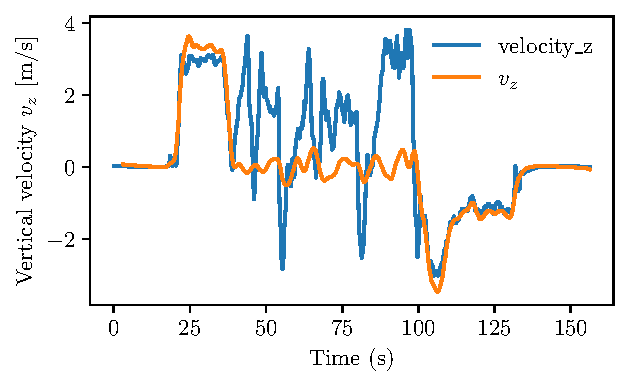
\includegraphics[width=0.9\linewidth]{figures/vz_different_ways.pdf}
    \caption{Vertical velocity versus time: comparison between given and calculated vertical velocity.}
    \label{fig:vz_diff_ways}
\end{figure}
% 
The horizontal speed $v$ was computed from the velocity components using the Euclidean norm as shown in Eq.~\eqref{eq:v}:
\begin{equation}
v = \sqrt{v_x^2 + v_y^2}  
\label{eq:v}
\end{equation}
% 
Here, $v_x$ and $v_y$ are velocities in $x$ and $y$-directions, respectively. 
Finally, the battery power was computed from voltage and current measurements as shown in Eq.~\eqref{eq:P}:
\begin{equation}
P_{\text{real}} = V_{\text{battery}} \cdot I_{\text{battery}} 
\label{eq:P}
\end{equation}
where $ P_{\text{real}} $ is the instantaneous power in watts, $ V_{\text{battery}} $ is the measured battery voltage, and $ I_{\text{battery}} $ is the measured battery current.

\subsection{Data analysis}
To better understand the aircraft’s motion prior to flight-phase classification, histograms of vertical velocity, horizontal velocity, and power were analyzed. Figure~\ref{fig:vz_hist} illustrates the histogram of the derived vertical velocity $v_z$, which displays a dominant peak near zero associated with cruise or level flight. Deviations from zero form two clear tails, indicating ascent and descent.
\begin{figure}[h]
    \centering
    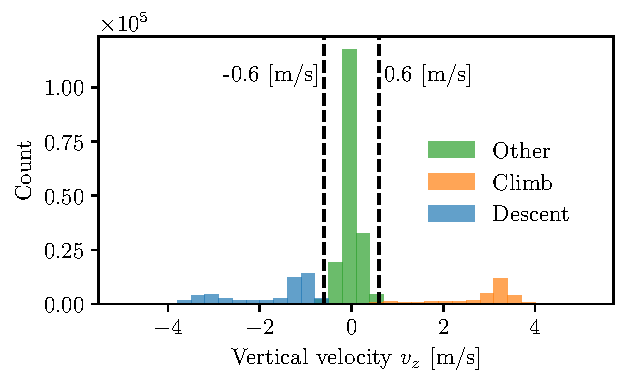
\includegraphics[width=0.9\linewidth]{figures/vertical_speed_histogram_by_phase.pdf}
    \caption{Distribution of vertical velocity as a histogram.}
    \label{fig:vz_hist}
\end{figure}
The threshold values of $\pm 0.6$~m/s were selected to define flight phases in the next section. The clear separation observed in the histogram supports different flight phase classification.

\begin{figure}[h]
    \centering
    
\includegraphics[width=0.9\linewidth]{figures/horizontal_speed_hist.pdf}
    \caption{Distribution of horizontal speed as a histogram.}
    \label{fig:v_hist}
\end{figure}
In addition to vertical motion, the horizontal speed was analyzed to further characterize the flight behavior. Figure~\ref{fig:v_hist} illustrates the histogram of the horizontal speed $v$. The distribution is strongly skewed toward low speeds, indicating that a large portion of the flight time is spent in hovering, takeoff, landing, or slow maneuvering conditions. A threshold value of $0.3$~m/s was selected to distinguish hovering from forward flight. Horizontal speeds below this threshold are classified as no forward motion. At higher speeds, the histogram exhibits multiple peaks, which correspond to different predefined forward-flight velocities. 

Finally, the power consumption was analyzed to capture the energetic characteristics of different flight conditions. Figure~\ref{fig:power_hist} shows the histogram of the measured battery power $P_{\text{real}}$, which exhibits a strong concentration at low power values corresponding to idle, hovering, or ground operation, along with a broader peak at higher power levels associated with active flight. Based on this distribution, a threshold value of 50~W was selected to distinguish between low-power and active-flight regimes. This threshold is consistent with findings by \cite{patterson2018}, who report that power during ground operations is approximately 10\% of that during cruise flight.

\begin{figure}
    \centering
    
\includegraphics[width=0.9\linewidth]{figures/power_his.pdf}
    \caption{Distribution of battery power measured as a histogram.}
    \label{fig:power_hist}
\end{figure}


% \section{Data analysis}
% 

The raw flight data from the DJI~100 were reviewed and cleaned before analysis to check for errors and unrealistic values. All flight identifiers and time fields were converted into consistent formats, and a single timestamp was created from the recorded date and time. The data were then sorted chronologically for each flight and checked for duplicate records.

Physical range limits were applied to the telemetry variables based on the expected operating conditions of the DJI~100. These limits included a maximum wind speed of 60~m/s, battery voltage between 5 and 30~V, battery current within $\pm 500$~A, velocity limited to 50~m/s, total speed limited to 100~m/s, acceleration limited to 100~m/s$^2$, angular rate limited to 50~rad/s, altitude constrained between $-100$~m and 5{,}000~m, and position values restricted to a reasonable spatial bound. Orientation data were also checked to ensure that quaternion norms remained close to one. As a results, no data points were removed, indicating that the dataset was already clean and within the expected physical limits.\\

After cleaning the data using predefined physical limits, the measured altitude was redefined relative to the initial altitude of each flight. The relative altitude $z(t)$ in  Eq.~\eqref{eq:zt} was computed by subtracting the altitude at the start of the flight from the measured altitude at each time step.\\
\begin{equation}
    z(t) = \text{altitude}(t) - \text{altitude}(t=0)
    \label{eq:zt}
\end{equation}
where $ z(t) $ is the relative altitude at time $ t $.
Using this relative altitude, the vertical velocity was then derived by computing the rate of change of altitude with respect to time
using Eq.~\eqref{eq:vz} and to reduce noise in the vertical velocity signal, a one-dimensional Gaussian filter was  also applied to the vertical velocity  $v_z$  within each flight.\\
\begin{equation}
v_{z}(t) = \frac{dz(t)}{dt}
\label{eq:vz}
\end{equation}
This derived velocity was compared with the recorded vertical velocity $\texttt{velocity\_z}$ provided in the dataset. As shown in Fig.~\ref{fig:vz_diff_ways}, although both  velocities follow similar overall trends, the $\text{velocity\_z}$ exhibits larger fluctuations, while  $v_z$ is smoother, particularly during the cruise phase of flight. These differences are likely caused by sensor noise, measurement delays, or onboard filtering effects. The observed inconsistencies also suggest a possible error in the \texttt{velocity\_z} column, which is most likely associated with the drone’s orientation rather than true vertical motion. Therefore, all further data analysis was performed using the vertical velocity derived from altitude, $v_z$.

The horizontal speed $v$ was computed from the velocity components using the Euclidean norm as shown in Eq.~\eqref{eq:v} :
\begin{equation}
v = \sqrt{v_x^2 + v_y^2}  
\label{eq:v}
\end{equation}

Finally, the battery power was computed from voltage and current measurements as shown in Eq.~\eqref{eq:P}:
\begin{equation}
P_{\text{real}} = V_{\text{battery}} \cdot I_{\text{battery}} 
\label{eq:P}
\end{equation}
where $ P_{\text{real}} $ is the instantaneous power in watts, $ V_{\text{battery}} $ is the measured battery voltage, and $ I_{\text{battery}} $ is the measured battery current.\\

To better understand the aircraft’s motion prior to flight-phase classification, histograms of vertical velocity, horizontal velocity, and power were analyzed. Figure~\ref{fig:vz_hist}
 illustrates the histogram of the derived vertical velocity $v_z$, which displays a dominant peak near zero associated with cruise or level flight. Deviations from zero form two clear tails, indicating ascent and descent.
The threshold values of $\pm 0.6$~m/s were selected to define flight phases. Vertical velocities greater than $0.6$~m/s are classified as climb, as a true ascent require a positive vertical velocity, while values below $-0.6$~m/s indicate descent. Vertical velocities within this range are classified as cruise, allowing for small fluctuations around zero caused by sensor noise or minor altitude adjustments. The clear separation observed in the histogram supports different  flight phase classification.

In addition to vertical motion, the horizontal speed was analyzed to further characterize the flight behavior. Figure~\ref{fig:v_hist} illustrates the histogram of the horizontal speed $v$. The distribution is strongly skewed toward low speeds, indicating that a large portion of the flight time is spent in hovering, takeoff, landing, or slow maneuvering conditions.A threshold value of $0.3$~m/s was selected to distinguish hovering from forward flight. Horizontal speeds below this threshold are classified as hovering, while speeds above $0.3$~m/s indicate forward motion. At higher speeds, the histogram exhibits multiple peaks, which likely correspond to different forward-flight regimes or mission segments.\\
Finally, the power consumption was analyzed to capture the energetic characteristics of different flight conditions. Figure~\ref{fig:power_hist} shows the histogram of the measured battery power $P_{\text{real}}$, which exhibits a strong concentration at low power values corresponding to idle, hovering, or ground operation, along with a broader peak at higher power levels associated with active flight. Based on this distribution, a threshold value of 50~W was selected to distinguish between low-power and active-flight regimes: power values below 50~W indicate non-flying or minimal-load conditions, while higher values correspond to sustained flight and maneuvering. The clear separation between these regions in the histogram supports the use of power as an additional indicator for flight phase identification.

.







\begin{figure}
    \centering
    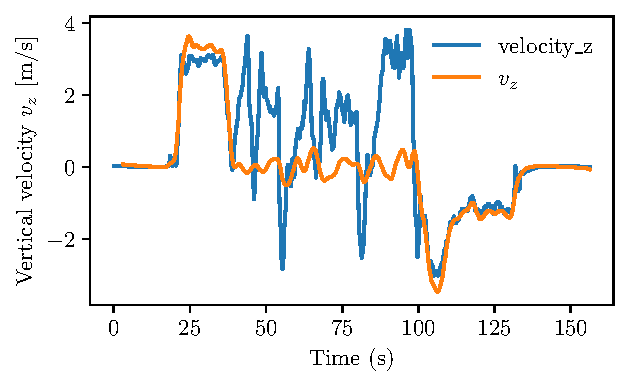
\includegraphics[width=0.9\linewidth]{figures/vz_different_ways.pdf}
    \caption{Caption}
    \label{fig:vz_diff_ways}
\end{figure}
\begin{figure}
    \centering
    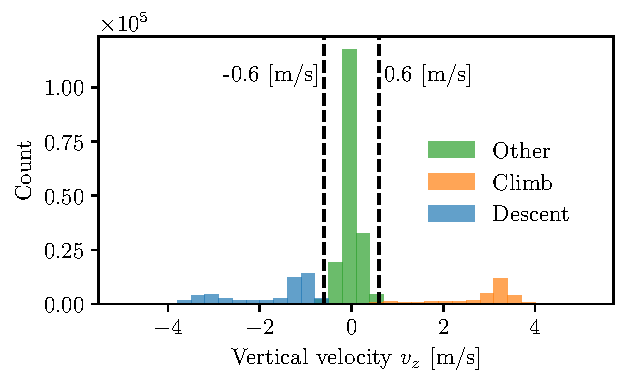
\includegraphics[width=0.9\linewidth]{figures/vertical_speed_histogram_by_phase.pdf}
    \caption{Caption}
    \label{fig:vz_hist}
\end{figure}
\begin{figure}
    \centering
    
\includegraphics[width=0.9\linewidth]{figures/horizontal_speed_hist.pdf}
    \caption{Caption}
    \label{fig:v_hist}
\end{figure}
\begin{figure}
    \centering
    
\includegraphics[width=0.9\linewidth]{figures/power_his.pdf}
    \caption{Caption}
    \label{fig:power_hist}
\end{figure}



\section{Definition of Flight Phases}
\label{flight_phases}
The flight phases for the DJI M100 are defined based on motion and altitude thresholds as follows:

\subsection{Taxi Phase}
The \textit{Taxi} phase corresponds to a low-motion state characterized by negligible horizontal and vertical movement, accompanied by minimal power consumption. This phase typically occurs during ground operations, such as taxiing on runways or moving between takeoff and landing positions. A flight segment is classified as \textit{Taxi} if and only if all of the following conditions are satisfied:
\begin{equation}
v < 0.3 \quad \land \quad \left| v_z \right| < 0.2 \quad \land \quad P_\text{real} < 50.0.    
\end{equation}

The logical conjunction ($\land$) ensures that all three conditions must hold simultaneously for classification.

\subsection{Hover Phase}
The \textit{Hover} phase denotes a state of stable, near-stationary flight in both horizontal and vertical dimensions. Unlike the \textit{Taxi} phase, power consumption may be significant due to the sustained lift required to maintain altitude. This phase is typical during aerial inspection, target tracking, or waiting maneuvers. A segment is classified as \textit{Hover} if and only if:
\begin{equation}
v < 0.3 \quad \land \quad \left| v_z \right| < 0.2.
\end{equation}

\subsection{Cruise Phase}
The \textit{Cruise} phase represents steady, forward flight at a stable altitude, typical of long-range or efficient flight operations. This phase is characterized by minimal vertical motion and flight at a significant fraction of the maximum achievable altitude. A segment is classified as \textit{Cruise} if and only if:
\begin{equation}
\left| v_z \right| < 0.6 \quad \land \quad z > 0.8 \times \text{max}(z).    
\end{equation}

\subsection{Climb Phase}
The \textit{Climb} phase is defined by a positive vertical velocity exceeding the cruise threshold, indicating active ascent. This phase is critical for assessing energy expenditure during altitude gain. A segment is classified as \textit{Climb} if and only if:
\begin{equation}
v_z > 0.6.    
\end{equation}

\subsection{Descent Phase}
The \textit{Descent} phase corresponds to a controlled or uncontrolled downward trajectory, characterized by a vertical velocity below the negative cruise threshold. This phase is essential for analyzing landing procedures and energy recovery. A segment is classified as \textit{Descent} if and only if:
\begin{equation}
v_z < -0.6.    
\end{equation}

\subsection{Other Phase}
The \textit{Other} phase serves as a default category for all data points that do not satisfy the conditions of the above five phases. This includes transitional states (e.g., from hover to climb, or during abrupt maneuvers), invalid or corrupted data, and anomalous flight behaviors. Formally, a segment belongs to the \textit{Other} phase if it fails to satisfy the conjunction of conditions defining any of the preceding phases.

\subsection{Sample flight trajectory}
Based on the previously defined criteria for different flight phases,  Figure~\ref{fig:phase_seg_01} presents a representative example demonstrating how these phases are identified in practice using real flight data. The figure shows the trajectory of flight~79 , where the x-axis represents time, the left y-axis indicates height, and the right y-axis shows velocity. The height profile is shown by the blue curve, while the vertical speed and horizontal speed are represented by the red and green curves, respectively. The background shading indicates classified flight phases, including taxi, climb, cruise, descent, hover, and other.

At the beginning of the mission (0--20~s), the vehicle remains at ground level with near-zero vertical speed, corresponding to the taxi phase. Between approximately 20~s and 40~s, the height increases rapidly and the vertical speed becomes positive, indicating the climb phase. From about 40~s to 95~s, the vehicle maintains an approximately constant height of around 50~m, which corresponds to the cruise phase. During this interval, the vertical speed remains close to zero, while the horizontal speed is relatively high and exhibits noticeable oscillations, likely due to maneuvering or control adjustments. At around 95~s, the height begins to decrease and the vertical speed becomes negative, marking the start of the descent phase, which continues until the vehicle reaches ground level at approximately 130~s. Finally, from 130~s to 160~s, the vehicle remains on the ground with near-zero height and velocities, returning to the taxi phase. Overall, the figure demonstrates a complete mission profile and highlights the consistency between the kinematic variables and the identified flight phases. Figure \ref{fig:phase_seg_02} illustrates the temporal variation of wind speed and corresponding power consumption.


\begin{figure*}
    \centering
    
\includegraphics[width=0.9\linewidth]{figures/phases_plot.pdf}
    \caption{Time series of drone altitude, vertical speed, and horizontal speed for flight 79, with segments colored by flight phase (as per legend).}
    \label{fig:phase_seg_01}
\end{figure*}
\begin{figure*}
    \centering
    
\includegraphics[width=0.9\linewidth]{figures/phases_power_plot.pdf}
    \caption{Time series of wind speed, and power measured for flight 79, with segments colored by flight phase (as per legend in Figure \ref{fig:phase_seg_01}).}
    \label{fig:phase_seg_02}
\end{figure*}




\section{Physical model}
\label{Physic_model}
In this section, we develop a simple analytical physics-based model that relates the electrical power consumption of a multirotor UAV to its mass, thrust generation, climb and descent rate, aerodynamic drag, and environmental wind conditions. The model follows a quasi-steady flight assumption, which is commonly adopted in UAV energy modeling \cite{lieshman2006, hwang2018}.

\subsection{Hover Power}

The DJI Matrice 100 is a quadrotor UAV equipped with four identical counter-rotating rotors, each modeled as an actuator disk with radius $ R = 0.165~\text{m} $. The total rotor disk area $A_{\text{tot}}$ is given by:
\begin{equation}
A_{\text{tot}} = N \pi R^2 = 4 \pi R^2,
\end{equation}
where $ N = 4 $ is the number of rotors.

In hover flight, the induced velocity $ v_h $, the downward velocity of air through the rotor disk, is derived from momentum theory:
\begin{equation}
v_h = \sqrt{\frac{mg}{2 \rho A_{\text{tot}}}},
\end{equation}
where:
\begin{itemize}
    \item $ m = M_0 + \text{payload\_kg} $ is the total mass of the UAV (including empty mass $ M_0 = 3.68~\text{kg} $ and payload),
    \item $ g = 9.81~\text{m/s}^2 $ is the gravitational acceleration,
    \item $ \rho = 1.225~\text{kg/m}^3 $ is the air density at sea level.
\end{itemize}

The ideal mechanical power required to sustain hover, neglecting profile and parasitic losses, is:
\begin{equation}
P_{\text{hover}} = \frac{W^{3/2}}{\sqrt{2 \rho A_{\text{tot}}}},
\end{equation}
where $ W = mg $ is the weight of the UAV. This expression assumes ideal actuator disk theory and is used as a baseline for estimating power requirements in vertical flight \cite{lieshman2006, johnson1980, gong2022}.

\subsection{Climb and descent Power}
For vertical flight, the induced power is corrected using axial momentum theory
\begin{equation}
    P_\text{induced} = P_\text{hover} \cdot \left [  \frac{v_z}{v_h} + \frac{v_i}{v_h} \right ] ,
\end{equation}
where,
\begin{equation}
    \frac{v_i}{v_h} = - \left ( \frac{v_z}{2v_h} \right ) + \sqrt{ \left ( \frac{v_z}{2v_h} \right )^2 + 1 }.
\end{equation}
This gives
\begin{equation}
P_{\text{induced}} = P_\text{hover} \left [ \frac{v_z}{2v_h} +\sqrt{ \left ( \frac{v_z}{2v_h} \right )^2 + 1 } \right]    .
\end{equation}
where $v_z >0$ corresponds to climb and $v_z < 0$ to descent. This formulation captures the increased power demand during climb and reduced induced power during descent while avoiding non-physical negative power values \cite{lieshman2006, johnson1980}.

\subsection{Cruise}
The aerodynamic drag force is modeled as
\begin{equation}
P_{\text{drag}} = \frac{1}{2} \rho C_d S_{\text{ref}} v_{\text{air}}^3    
\end{equation}
Here, $v_{\text{air}}$ is relative velocity between drone and wind, $C_d$ is the drag coefficient and $S_{\text{ref}}$ is the reference area.

Analysis of the onboard attitude quaternion data shows that the pitch angle of the UAV is strongly concentrated around $0$ degree, indicating predominantly near level flight conditions. Under near-level flight conditions, the aerodynamic drag characteristics of multirotor UAVs can be approximated using drag coefficients reported for zero or near-zero fuselage pitch angles. Following the experimental study \cite{hammer2024}, an effective drag coefficient of $C_d = 0.32$ is adopted.

In the same study, the authors approximate the aerodynamic reference area for small multirotor UAVs with a total mass in the range of 3–4 kg using an effective frontal reference area \cite{hammer2024}. Accordingly, for the DJI Matrice 100 platform with a total mass of approximately 3.6 kg, the reference area is adopted as
$S_{\text{ref}} = 0.05 ~\text{m}^2$.

The total mechanical power during cruise is approximated as
\begin{equation}
P_{\text{cruise}} = P_{\text{hover}} + P_{\text{drag}}
\end{equation}

\subsection{Segment-Wise Efficiency Estimation}

To better capture the dynamic nature of UAV propulsion losses across different flight regimes, a segment-wise efficiency estimation approach is adopted, replacing the assumption of a single constant efficiency. The electrical power drawn from the battery is related to the mechanical power output by:
\begin{equation}
P_{\text{battery}} = \frac{P_{\text{mech}}}{\eta},
\end{equation}
where $\eta$ denotes the effective system efficiency, representing the aggregate losses across the propulsion chain, including electric motors, electronic speed controllers, propellers, and electrical wiring. By estimating $\eta$ separately for distinct flight segments, the model accounts for varying dominant loss mechanisms \cite{jacewicz2022}.

Efficiency values are identified from given flight data by analyzing the ratio of mechanical power to electrical power. The results reveal significant variation across flight phases:

\begin{itemize}
    \item \textbf{Hover:} $\eta = 0.83$ — Highest efficiency due to stable, symmetric induced flow and minimal parasitic drag. Power is primarily used to generate lift, with relatively low aerodynamic losses.
    
    \item \textbf{Cruise:} $\eta = 0.46$ — Marked reduction in efficiency caused by increased parasite drag, higher airspeed-induced losses, and non-optimal propeller inflow conditions in forward flight.
    
    \item \textbf{Climb:} $\eta = 0.53$ — Moderate efficiency reflecting the additional power required to overcome gravity, combined with increased induced and profile losses due to higher thrust demand.
    
    \item \textbf{Descent:} $\eta = 0.61$ — Efficiency improves compared to climb, as the induced power requirement decreases and the UAV may benefit from partial energy recovery (e.g., regenerative braking in some systems), though this effect is typically limited in standard quadrotors.
\end{itemize}

\subsection{Model Evaluation}

The proposed physics-based propulsion model is evaluated by comparing predicted electrical power consumption against measured flight data across distinct flight segments, excluding transitional phases. Performance is quantified using three error metrics: Mean Absolute Error (MAE), Root Mean Square Error (RMSE), and Mean Absolute Percentage Error (MAPE), as summarized in Table~\ref{tab:error_by_segment}

\begin{table}[tbhp]
\centering
\caption{Error by Segment (Excluding Transition)}
\label{tab:error_by_segment}
\begin{tabular}{lrrrr}
\textbf{Segment} & \textbf{MAE (W)} & \textbf{RMSE (W)} & \textbf{MAPE (\%)} \\
Hover      & 185.36 & 196.14 & 84.86 \\
Climb      & 56.99  & 82.64  & 10.48 \\
Descent    & 45.71  & 64.36  & 9.58 \\
Cruise     & 54.79  & 73.81  & 11.01 \\
\end{tabular}
\end{table}

The results indicate strong performance in cruise, climb, and descent phases, with MAPE values below 12\% and RMSE under $85~\text{W}$, suggesting relatively accurate modeling of aerodynamic and propulsion dynamics under steady forward and vertical motion. The higher MAPE in hover (84.86\%) is attributed to the high sensitivity of power to small variations in thrust and induced velocity, as well as the dominance of induced power and inherent inefficiencies in the rotor system. Overall, the segment-wise efficiency approach significantly improves fidelity, demonstrating the value of phase-dependent modeling in UAV performance estimation.


\section{Random Forest Model for Power Prediction}
\label{data_driven}
Random Forest is an ensemble learning method that constructs multiple decision trees during training and outputs the average prediction (for regression) to improve accuracy and reduce overfitting \cite{gora2022}. Each tree is trained on a random subset of the data (bootstrap sampling) and a random subset of features at each split, enhancing model robustness and generalization.

In this study, a Random Forest Regressor from \texttt{scikit-learn} \cite{scikit} was used to predict UAV power consumption (\texttt{power\_w}) based on 19 features: \texttt{wind\_speed}, \texttt{wind\_angle}, \texttt{roll}, \texttt{pitch}, \texttt{yaw}, \texttt{velocity\_x}, \texttt{velocity\_y}, \texttt{velocity\_z}, \texttt{vz\_from\_alt}, \texttt{angular\_x}, \texttt{angular\_y}, \texttt{angular\_z}, \texttt{linear\_acceleration\_x}, \texttt{linear\_acceleration\_y}, \texttt{linear\_acceleration\_z}, and binary flight mode indicators (\texttt{is\_cruise}, \texttt{is\_climb}, \texttt{is\_descent}, \texttt{is\_hover}). 
To extract the corresponding Euler angles, roll ($\phi$), pitch ($\theta$), and yaw ($\psi$), the transformation from quaternion to Euler angles is derived from the relationship between rotation matrices and quaternions, and is given by the following equations:

\begin{align}
\phi &= \operatorname{atan2}(2(w x + y z), 1 - 2(x^2 + y^2)), \\
\theta &= \operatorname{arcsin}(2(w y - z x)), \\
\psi &= \operatorname{atan2}(2(w z + x y), 1 - 2(y^2 + z^2)).
\end{align}

To ensure numerical stability, the input quaternion was normalized prior to conversion. In cases where the pitch angle approached $\pm \pi/2$, the $\operatorname{arcsin}$ function was clamped to $\pm \pi/2$ to prevent gimbal lock artifacts. The resulting Euler angles were computed for each time step in \texttt{pandas} \cite{pandas}.

The model was trained on a 80–20 train-test split with hyperparameters tuned via cross-validation. It achieved an R$^2$ score of 0.941, demonstrating strong predictive performance. Feature importance analysis identified \texttt{velocity\_z}, \texttt{wind\_speed}, and flight mode variables as the most influential predictors, consistent with physical expectations of power demand during vertical motion and environmental interaction.

\subsection{Model Evaluation}

Model performance is again quantified using MAE, RMSE, and MAPE, as summarized in Table~\ref{tab:performance_no_transition}.

\begin{table}[hp]
\centering
\caption{Model performance by flight mode (Random Forest).}
\label{tab:performance_no_transition}
\begin{tabular}{lrrrr}
\textbf{Segment} & \textbf{MAE (W)} & \textbf{RMSE (W)} & \textbf{MAPE (\%)} \\
Hover      & 46.69 & 74.98 & 20.60 \\
Climb      & 33.39 & 46.40 & 6.17 \\
Descent    & 33.37 & 46.92 & 7.21 \\
Cruise     & 37.14 & 49.21 & 7.46 \\
\end{tabular}
\end{table}

The Random Forest model demonstrates strong predictive accuracy across all flight modes. Notably, it achieves significantly lower errors compared to the physics-based model in hover, with MAPE reduced from 84.86\% to 20.60\%, indicating its ability to capture complex, non-linear relationships in induced power and system inefficiencies. The model maintains low MAPE values (below 8\%) in climb, descent, and cruise, reflecting its robustness in steady-state flight regimes. 


\section{Model validation and comparison}
\label{task_04}
\subsection{Transient Response Analysis}
\begin{figure*}[tph]
    \centering
    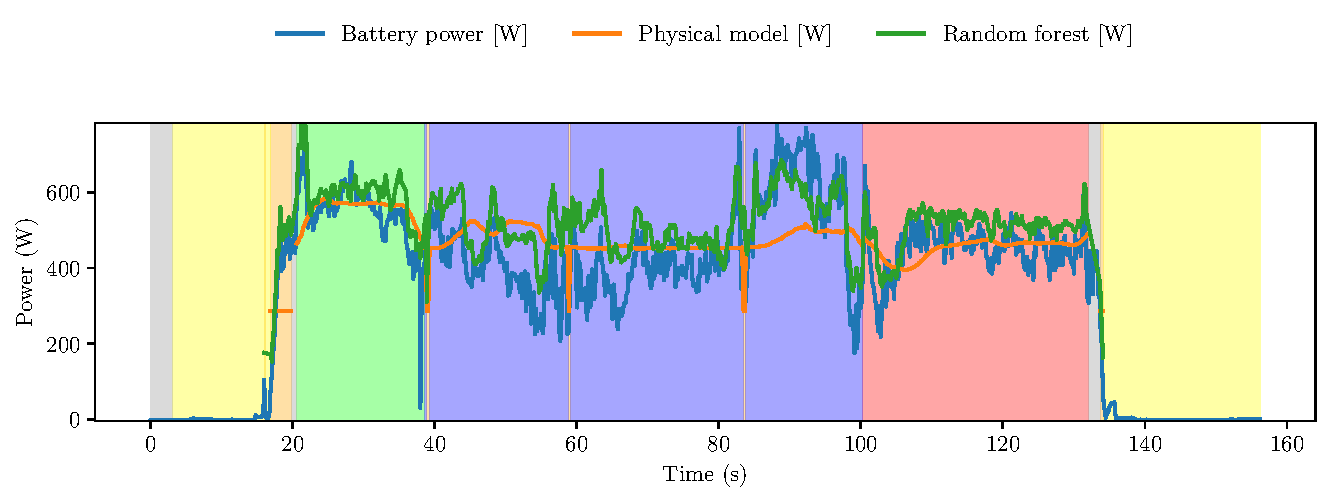
\includegraphics[width=0.9\linewidth]{figures/phases_power_compare.pdf}
    \caption{Dynamic (transient) response of both models versus real-time power consumption during flight 79. Flight segments are colored by flight phase as per legend in Figure \ref{fig:phase_seg_01}.}
    \label{fig:phase_power_comp}
\end{figure*}
To assess the models’ ability to capture short-term power dynamics, the predicted and measured power trajectories of the representative flight $79$ are compared in Figure~\ref{fig:phase_power_comp}. The time series spans critical operational phases—taxi, climb, cruise, descent, and hover—providing a detailed view of model behavior during transitions and high-dynamic maneuvers. Measured power exhibits pronounced fluctuations during climb and cruise, driven by rapid changes in thrust, drag, and control inputs. The physics-based model generates smooth, continuous predictions that follow the general trend but consistently lags behind or underestimates transient peaks and dips, indicating a limited ability to respond to sudden changes. In contrast, the Random Forest model closely tracks the measured power across all phases, accurately replicating rapid variations in response to flight dynamics and environmental conditions. This superior temporal fidelity highlights the model’s strength in learning complex, time-varying interactions from historical data. Unlike analytical models constrained by fixed equations, the Random Forest approach adapts to real-world nuances such as control effort, wind gusts, and maneuver intensity. These findings underscore a key advantage of data-driven methods: their capacity to model transient behavior and operational subtleties that are difficult or impossible to encode in physics-based formulations. 

\subsection{Quantitative Performance Comparison}

Now, the two models—Random Forest and the physics-based model—are evaluated using standard error metrics: MAE, RMSE, and MAPE. As illustrated in Figure~\ref{fig:model_comp}, the Random Forest model achieves a consistent improvement of approximately 45–50\% across all metrics compared to the physics-based approach. 
\begin{figure}[h]
    \centering
    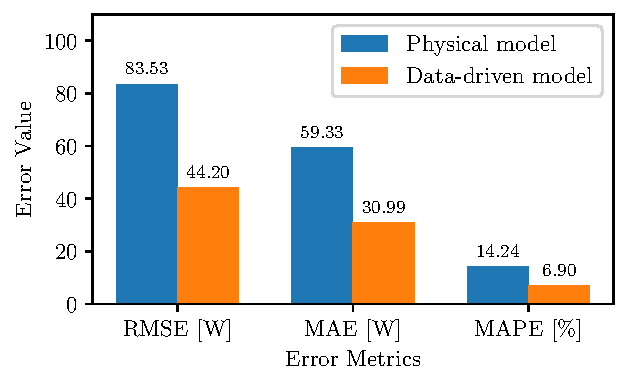
\includegraphics[width=0.9\linewidth]{figures/model_comparison.pdf}
    \caption{Performance comparison of the two models based on various error metrics.}
    \label{fig:model_comp}
\end{figure}
This substantial gain aligns with recent findings in the literature \cite{zhang2021}, which emphasize the inherent limitations of physics-driven models in complex, real-world scenarios. While such models can capture broad trends in power consumption based on aerodynamic and propulsion principles, they often fail under dynamic flight conditions due to simplifying assumptions, unmodeled nonlinearities, and sensitivity to parameter uncertainty \cite{dorling2017}. In contrast, the Random Forest model, trained on a large dataset of real flight observations, effectively learns the intricate, non-linear dependencies between flight states (e.g., speed, acceleration, payload) and energy demand. This data-driven capability enables significantly higher prediction accuracy, particularly in variable or high-dynamic regimes. The results reinforce the growing consensus that machine learning methods outperform traditional physics-based models in terms of numerical precision and robustness, making them better suited for accurate energy estimation in practical UAV operations \cite{muli2022}.


\subsection{Interpretability and generalisation}
Interpretability refers to the degree to which the influence of input variables on model predictions can be understood and explained. Physics-based models are grounded in well-established analytical equations derived from fundamental principles of aerodynamics, mechanics, and thermodynamics. This inherent transparency allows for direct physical interpretation of model outputs. In contrast, Random Forest model, comprising ensembles of decision trees, operate through complex, non-linear statistical learning processes. While feature importance analysis can provide partial insight into which inputs most influence predictions, the internal decision logic remains opaque and difficult to trace. As a result, data-driven models offer only moderate interpretability, limiting their utility in safety-critical applications where explainability is paramount \cite{zhang2021, muli2022, gora2022}.

Generalization is the ability of a model to maintain accuracy when applied to unseen flight conditions or new UAV platforms. It is a critical factor in real-world deployment. To evaluate this, we conducted a sensitivity test by modifying the linear acceleration of a representative flight beyond the range observed in the training data. The resulting energy consumption (calculated according to Eq. \ref{eq:energy}) trend is shown in Figure~\ref{fig:generalisation}, where the Random Forest model incorrectly predicts a decrease in energy consumption with increasing acceleration. This is an unphysical behavior. This contrasts sharply with the expected trend observed within the training regime (Figure~\ref{fig:energy_vs_az}), where energy consumption increases with acceleration, consistent with real-world dynamics. The model’s erroneous extrapolation highlights a key limitation: Random Forests lack the ability to generalize reliably outside the domain of their training data. 

\begin{figure}[h]
    \centering
    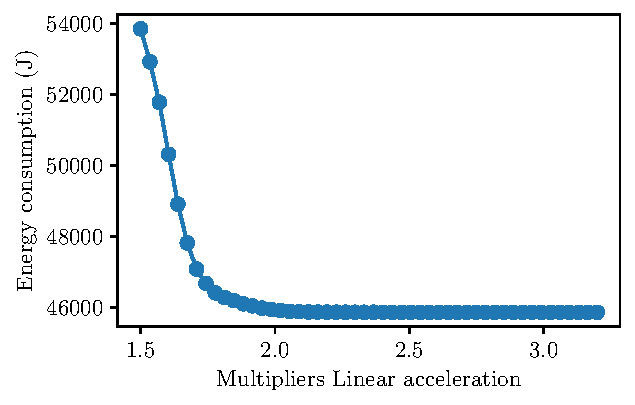
\includegraphics[width=0.9\linewidth]{figures/Energy_vs_az_generalisation.pdf}
    \caption{Sensitivity of ML model to linear acceleration values outside the training data range.}
    \label{fig:generalisation}
\end{figure}
Both physics-based and data-driven models exhibit strong performance when operating within the range of conditions present in their training data \cite{zhang2021}. Physics-based models may require manual recalibration of physical parameters (e.g. drag coefficients, motor efficiency) when applied to different platforms or environments \cite{hwang2018}. Similarly, data-driven models often fail to extrapolate correctly and may produce physically implausible results when pushed beyond their training boundaries. These findings underscore a fundamental trade-off: while physics-based models offer superior interpretability, and data-driven models deliver higher accuracy within their domain, neither approach ensures robust performance across all operational scenarios without additional adaptation. 


\section{Application to Energy-aware mission planning}
\label{task_05}
Flight 79 is selected as a representative case for the energy consumption analysis. This flight includes multiple operational phases such as take-off, climb, cruise, maneuvering, and descent, which makes it suitable for evaluating energy behavior under realistic mission conditions. 

For Flight 79, instantaneous power consumption is predicted using the trained Random Forest regression model as mentioned earlier. The total energy consumption of Flight 79 is computed by integrating power over time. 

\begin{equation}
E = \int_{t_1}^{t_2} P(t)  dt    
\label{eq:energy}
\end{equation}

The integration was carried out numerically by using the trapezoidal rule. The measured energy serves as a reference value, while the predicted energy represents the model’s estimate for the same flight under identical operating conditions. 
The integrated energy corresponding to the measured power of Flight 79 is defined as the baseline energy consumption. This baseline value is later used as a reference point for sensitivity analyses, where specific mission parameters such as wind speed, payload, and linear acceleration are varied while keeping all other flight characteristics unchanged.

\subsection{Effect of wind speed on energy consumption}
To evaluate the sensitivity of energy consumption to wind conditions, the recorded wind speed of Flight 79 is systematically scaled using multiplicative factors ranging from 0.5 to 2.0. For each wind speed scaling factor, the Random Forest model predicts the instantaneous power consumption over the entire flight duration. The predicted power signal is then integrated over time to obtain the corresponding total energy consumption. 

\begin{figure}[tph]
    \centering
    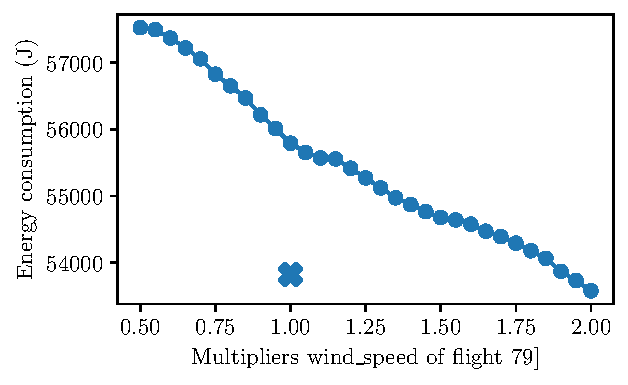
\includegraphics[width=0.9\linewidth]{figures/energy_vs_wind_speed.pdf}
    \caption{Energy consumption as a function of wind speed.}
    \label{fig:energy_vs_wind}
\end{figure}

Figure \ref{fig:energy_vs_wind} presents the predicted total energy consumption
as a function of the wind speed multiplier. The crossed marker at a multiplier of 1.0 indicates the baseline energy consumption corresponding to the measured power consumption. The observed trend shows a decrease in energy consumption with increasing wind speed, which initially appears counterintuitive. However, further analysis revealed that the wind was coming from behind the drone (tailwind), reducing aerodynamic drag and aiding forward motion. As a result, the UAV required less power, leading to lower energy consumption as wind speed increased.

\subsection{Effect of payload on energy consumption}
\begin{figure} [tph]
    \centering
    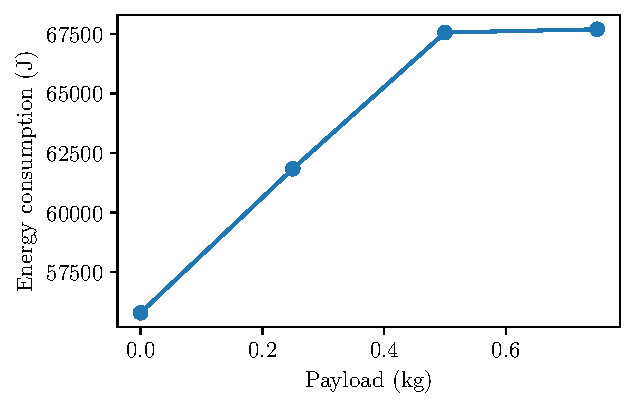
\includegraphics[width=0.9\linewidth]{figures/Energy_vs_payload.pdf}
    \caption{Energy consumption as a function of payload.}
    \label{fig:energy_vs_payload}
\end{figure}

To analyze the impact of payload on energy consumption, the payload mass is systematically varied while keeping all other flight parameters unchanged. 
Figure \ref{fig:energy_vs_payload} illustrates the relationship between payload mass and total energy consumption for Flight 79. The observed trend shows an increase in energy consumption with higher payload values, indicating the additional power required to sustain flight under increased mass. However, there is almost no observed increase in energy consumption when the payload is increased from 0.5 kg to 0.75 kg. This unexpected result is likely due to the limited training data available for the 0.75 kg payload. There are approximately 1,600 samples compared to around 80,000 samples for other payload levels i.e. 0 kg, 0.25 kg and 0.5 kg. As a result, the machine learning model’s ability to generalize and accurately predict energy behavior at 0.75 kg is significantly constrained, leading to unreliable predictions for this specific payload. 

\subsection{Effect of linear acceleration on energy consumption}
\begin{figure}[tph]
    \centering
    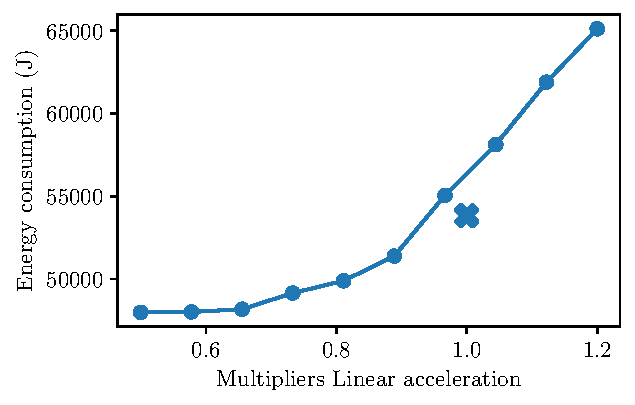
\includegraphics[width=0.9\linewidth]{figures/Energy_vs_az.pdf}
    \caption{Sensitivity of energy consumption to linear acceleration values in the training data range.}
    \label{fig:energy_vs_az}
\end{figure}

In addition to payload and wind effects, the influence of linear acceleration on energy consumption is evaluated to capture the impact of aggressive maneuvering and control effort. The linear acceleration components along the x, y, and z axes
of Flight 79 are scaled uniformly using multiplicative factors while keeping all other flight parameters unchanged. Figure \ref{fig:energy_vs_az} shows the variation in total energy consumption with increasing linear acceleration scaling. The increasing trend demonstrates that higher maneuvering intensity
leads to increased energy usage due to greater control effort and
propulsion demand.

\subsection{Feasibility analysis and return-to-home logic}
The predicted mission-level energy consumption obtained from the data-driven model enables a direct feasibility assessment for UAV operations. Using the sensitivity analyses presented in the previous sections, the effects of payload variation, wind speed scaling, and linear acceleration scaling on total mission energy consumption are quantified. Each scenario results in a modified energy estimate that represents the expected energy demand if the same trajectory were flown under altered conditions. These predicted energy values can be compared against the available onboard battery energy to assess mission feasibility. The Return-to-Home (RTH) decision logic can be formulated by comparing the predicted remaining energy required to complete the mission with the remaining battery capacity. If the estimated energy demand exceeds the available energy margin, the mission is classified as infeasible, and an RTH command can be triggered to ensure safe operation. Conversely, if sufficient energy margin exists, the mission may continue as planned. This framework demonstrates how the developed energy prediction models can be directly applied at the application level to support real-time decision-making. By continuously updating energy estimates based on changing payload, environmental conditions, and maneuver intensity, the UAV can autonomously assess mission feasibility and initiate safety actions when required.


\section{Summary and outlook}
This study presented a comprehensive framework for UAV energy consumption modeling, leveraging a publicly available dataset from 209 autonomous flights of a DJI Matrice 100 quadcopter collected over seven months under diverse operational and environmental conditions. A threshold-based flight phase classification scheme was developed, using histograms of vertical velocity, horizontal speed, and power consumption to define distinct segments i.e. Taxi, Hover, Cruise, Climb, Descent, and Other, ensuring robust and physically meaningful segmentation of flight data.
A physics-based power model was formulated using actuator disk theory and phase-dependent efficiency estimates. The model demonstrated consistent performance across hover, climb, descent, and cruise phases, with MAPE values below 12\% in cruise flight, confirming its ability to capture fundamental aerodynamic and propulsion dynamics under steady-state conditions.
A Random Forest regression model was trained on 19 flight-state features including velocity, wind, attitude, and flight mode indicators and achieved an
$R^2$ score of $0.941$, with MAE consistently below 50~W across all flight phases. The model significantly outperformed the physics-based approach, reducing prediction errors by up to 50\% and accurately tracking transient power variations during complex maneuvers.
However, the data-driven model exhibited unphysical extrapolation behavior when exposed to out-of-distribution conditions, and its internal decision logic remained opaque, limiting interpretability. In contrast, the physics-based model, while less accurate in dynamic regimes, maintained physical consistency and robustness beyond the training domain.
These results confirmed a fundamental trade-off: data-driven models offer superior accuracy within their training domain, but at the cost of generalization and explainability. Physics-based models, though less precise in complex scenarios, provide greater transparency and reliability under uncertainty. Future work should focus on improving the representation of the hover phase in physical models. To enhance generalization in data-driven approaches, models must be trained on diverse datasets that encompass a broad range of parameter values and operational scenarios.

\section*{Repository}
The source code, presentation, and report for this project are publicly available on GitHub. You can access the repository at:
\href{https://github.com/kanchanbansal-lab/Research_task}{https://github.com/kanchanbansal-lab/Research\_task}
The repository includes implementation details, model configurations, and data processing scripts.

\begin{thebibliography}{00}

\bibitem{muli2022}
Muli, Charles, Sanghyun Park, and Ming Liu. 2022.
“A Comparative Study on Energy Consumption Models for Drones.”
In \textit{Internet of Things (GIoTS 2022)},
edited by A. González-Vidal et al.,
Lecture Notes in Computer Science 13533.
Cham: Springer.

\bibitem{ren2025}
Ren, Guanting, Babar Shahzaad, Balsam Alkouz, Abdallah Lakhdari, and Athman Bouguettaya. 2026.
“Energy-Predictive Planning for Optimizing Drone Service Delivery.”
\textit{Expert Systems with Applications} 297 (Part A): 129251.
https://doi.org/10.1016/j.eswa.2025.129251.

\bibitem{zhang2021}
Zhang, Juan, James F. Campbell, Donald C. Sweeney II, and Andrea C. Hupman. 2021.
“Energy Consumption Models for Delivery Drones: A Comparison and Assessment.”
\textit{Transportation Research Part D: Transport and Environment} 90: 102668.
https://doi.org/10.1016/j.trd.2020.102668.

\bibitem{dorling2017}
Dorling, Kevin, Jörn Heinrichs, Geoffrey G. Messier, and Sebastian Magierowski. 2017.
“Vehicle Routing Problems for Drone Delivery.”
\textit{IEEE Transactions on Systems, Man, and Cybernetics: Systems} 47 (1): 70–85.

\bibitem{rodrigues2021}
Rodrigues, Thiago A., Jay Patrikar, Natalia L. Oliveira, H. Scott Matthews, Sebastian Scherer, and Constantine Samaras. 2021.
“In-Flight Positional and Energy Use Dataset of a DJI Matrice 100 Quadcopter for Small Package Delivery.”
\textit{Scientific Data} 8: 154.
https://doi.org/10.1038/s41597-021-00930-x.

\bibitem{rodrigues2022}
Rodrigues, Thiago A., Jay Patrikar, Natalia L. Oliveira, H. Scott Matthews, Sebastian Scherer, and Constantine Samaras. 2022.
“Drone Flight Data Reveal Energy and Greenhouse Gas Emissions Savings for Very Small Package Delivery.”
\textit{Patterns} 3 (8): 100569.
https://doi.org/10.1016/j.patter.2022.100569.

\bibitem{conte2022}
Conte, Carmelo, Giovanni Rufino, Gianluca de Alteriis, Vincenzo Bottino, and Domenico Accardo. 2022.
“A Data-Driven Learning Method for Online Prediction of Drone Battery Discharge.”
\textit{Aerospace Science and Technology} 130: 107921.
https://doi.org/10.1016/j.ast.2022.107921.

\bibitem{bruehl2021}
Brühl, Robert, Hartmut Fricke, and Michael Schultz. 2021.
“Air Taxi Flight Performance Modeling and Application.”

\bibitem{gora2022}
Gora, Kamil, Piotr Smyczynski, Mateusz Kujawinski, and Grzegorz Granosik. 2022.
“Machine Learning in Creating Energy Consumption Model for UAV.”
\textit{Energies} 15 (18): 6810.
https://doi.org/10.3390/en15186810.

\bibitem{lieshman2006}
Leishman, J. Gordon. 2006.
\textit{Principles of Helicopter Aerodynamics}.
Cambridge: Cambridge University Press.

\bibitem{johnson1980}
Johnson, Wayne. 1980.
\textit{Helicopter Theory}.
Princeton, NJ: Princeton University Press.

\bibitem{hwang2018}
Hwang, Seungmin, et al. 2018.
“Energy Consumption Modeling for Multirotor UAVs.”
\textit{Journal of Aircraft}.

\bibitem{gong2022}
Gong, Ankang, et al. 2022.
“Modeling Power Consumption of Multirotor UAVs.”
\textit{Aerospace Science and Technology}.

\bibitem{hammer2024}
Hammer, Martin, et al. 2024.
“Aerodynamic Drag Characteristics of Multirotor UAVs.”
\textit{Aerospace}.

\bibitem{jacewicz2022}
Jacewicz, Mateusz, et al. 2022.
“Energy Consumption Analysis of Quadrotor UAVs.”
\textit{Energies}.

\bibitem{patterson2018}
Patterson, Michael, K. Antcliff, and L. Kohlman. 2018.
“A Proposed Approach to Studying Urban Air Mobility Missions Including an Initial Exploration of Mission Requirements.”
In \textit{Proceedings of the AHS International 74th Annual Forum \& Technology Display}.

\bibitem{dji2016}
DJI. 2016.
\textit{DJI Matrice 100 User Manual}.
Shenzhen: DJI.

\bibitem{scikit}
Pedregosa, Fabian, Gaël Varoquaux, Alexandre Gramfort, Vincent Michel, Bertrand Thirion, Olivier Grisel, Mathieu Blondel, et al. 2011.
“Scikit-Learn: Machine Learning in Python.”
\textit{Journal of Machine Learning Research} 12: 2825–2830.

\bibitem{pandas}
McKinney, Wes. 2010.
“Data Structures for Statistical Computing in Python.”
In \textit{Proceedings of the 9th Python in Science Conference}, 51–56.

\bibitem{fatima2022}
Fatima, Syeda Kounpal, Manzar Abbas, Imran Mir, Faiza Gul, Suleman Mir, Nasir Saeed, Abdullah Alhumaidi Alotaibi, Turke Althobaiti, and Laith Abualigah. 2022.
“Data Driven Model Estimation for Aerial Vehicles: A Perspective Analysis.”
\textit{Processes} 10 (7): 1236.
https://doi.org/10.3390/pr10071236.


\end{thebibliography}
\vspace{12pt}

\end{document}